\documentclass[bwprint]{gmcmthesis}
\usepackage{amsmath}
\usepackage{subfig}
\usepackage{pdfpages}
\usepackage{float}
\usepackage{tikz}
\usetikzlibrary{arrows.meta}
\numberwithin{figure}{section}
\renewcommand{\thefigure}{\arabic{section}-\arabic{figure}} 
% \documentclass[withoutpreface,bwprint]{cumcmthesis}
% 去掉封面与编号页

\title{中国研究生数学建模竞赛论文标题}
\baominghao{No.00000001} %参赛队号
\schoolname{XX大学/学院}%学校名称
\membera{队员A} %队员A
\memberb{队员B} %队员B
\memberc{队员C} %队员C
\begin{document}
 \maketitle
 \begin{abstract}
第一段：针对自己选择的题目，说明自己用了什么方法来解决的（这类题属于哪种典型的问题），其中利用了哪些关键的算法，再说出自己的所建模型的创新点。没有创新点，也可以说自己所建的模型相比较于其它的是一个很好的方案。

第二段：问题一中，针对具体问题，进行分析和求解，几句话介绍自己是怎么解决的，有数字结果的也可以直接贴结果。

第三段：问题二中，类比于第二段。

第四段：问题三中，类比于第三段。

第五段：问题四中，类比于第四段。

第六段：如果有问题五，类比于第五段，没有就结束，也可以写一下团队的想法。






\keywords{针对具体的问题列一到两个关键字\quad  建模算法列出\quad }
\end{abstract}

%\pagestyle{plain}

%目录
\tableofcontents
\newpage

% 问题重述（可直接粘贴进 GMCM 模板正文；按模板格式自行调整章节编号）
\section{问题重述}

\subsection{问题背景}

无线通信系统借助正交频分复用（OFDM）技术，将连续的宽带频谱资源离散化为一系列相互正交的子载波单元，以实现多载波并行传输。在第 $k$ 个子载波上，接收信号可表示为
\begin{equation}
	y_k = h_k s_k + n_k \label{eq:siso}
\end{equation}
其中 $h_k$、$s_k$ 与 $n_k$ 分别为该子载波上的复信道系数、发送符号与加性噪声；信道系数 $h_k$ 的幅度与相位分别表征信道对信号的幅度缩放与相位旋转。为进一步提升链路传输速率，多输入多输出（MIMO）技术在收发两端配置多根天线，在空间域形成多个并行传输通道。本文所研究场景中，接收天线数为 $N_r=2$，发送天线数为 $N_t=4$，第 $k$ 个子载波上的信道矩阵为 $H_k\in\mathbb{C}^{2\times4}$，对应接收信号模型为 $y_k=H_k s_k+n_k$。在此基础上，发送波束赋形（TxBF）通过对各发送天线的信号施加相位旋转，利用电磁波的相干叠加原理将发送能量对准信道矩阵的主奇异值方向，从而获得额外的传输速率增益。

工程实践中，由于香农容量是理想条件下的理论上限，直接据此评估链路性能过于乐观，业界普遍采用物理层抽象方法对实际传输速率进行估计：首先计算各子载波上的信干噪比 $\mathrm{SINR}_k$，继而通过等效信干噪比映射（ESM）将 $K$ 个子载波的 SINR 降维为单一标量 $\mathrm{SINR}_{\mathrm{eff}}$，最后将其映射至实际传输速率档位（MCS 索引）。其中，指数有效信干噪比映射（EESM）是应用最为广泛的方法之一，其数学表达为
\begin{equation}
	\mathrm{SINR}_{\mathrm{eff}} = -\beta \ln\left( \frac{1}{K} \sum_{k=1}^{K} \exp\left( -\frac{\mathrm{SINR}_k}{\beta} \right) \right) \label{eq:eesm}
\end{equation}
其中 $\beta$ 为待拟合的模型参数，刻画了等效映射对信道频域选择性衰落的敏感程度。等效 SINR 映射的精度直接决定了链路速率估计的准确性，是物理层抽象技术的核心问题，也是本赛题关注的焦点。

\subsection{数据集说明}

赛题数据由网络设备在现网环境中采集：终端自预设起点依次移动至各目标点位并静止一段时间，设备在该过程中持续记录信道状态信息（CSI）与链路速率信息。采集数据按终端 MAC 地址组织为文件夹，每个文件夹包含训练集 A（Train）与测试集 B（Valid）两个目录。每条样本记录了维度为 $2\times4\times122$ 的 MIMO 信道矩阵（三个维度分别对应接收天线、发送天线与子载波数目），以及信道信息采集时间、速率信息采集时间、波束赋形开启指示与信道底噪等字段。训练集 A 额外包含实际传输速率标签：关闭 TxBF 场景下的 $r_{mcs}$ 与开启 TxBF 场景下的 $r_{mcs}^{bf}$；测试集 B 仅包含信道状态信息，不含速率标签。

\subsection{需要解决的问题}

\textbf{问题一：基于 EESM 的链路速率建模。}
利用训练集 A 中关闭 TxBF 场景下的实测 MIMO 信道数据 $H_{2\times4\times122}$ 及其对应的实际传输速率标签 $r_{mcs}$，对 EESM 模型的参数 $\beta$ 进行拟合；在此基础上，对测试集 B 中的信道数据依次完成：逐子载波 SINR 的计算、全部子载波 SINR 的等效 SINR 映射，以及链路传输速率索引 $r_{mcs}$ 的建模与估计。

\textbf{问题二：关闭 TxBF 场景下新型速率估计模型。}
针对关闭 TxBF 场景，在充分挖掘训练集 A 信道统计特征的基础上，突破传统 EESM 映射框架的局限，提出一种新的链路速率估计模型，并对测试集 B 中的信道数据估计其传输速率索引 $r_{mcs}$，力求取得优于 EESM 基线的估计精度。

\textbf{问题三：开启 TxBF 场景下新型速率估计模型。}
在开启 TxBF 场景下，发送信号经波束赋形后能量集中于信道矩阵主奇异值方向，等效信道的统计特性与关闭 TxBF 时存在显著差异。需针对该场景提出一种新的链路速率估计模型，利用训练集 A 进行模型训练，并对测试集 B 估计其传输速率索引 $r_{mcs}^{bf}$。


% 模型假设与符号说明（可直接粘贴进 GMCM 模板正文）
\section{模型假设}

\textbf{假设1（准静态信道假设）。}在每条信道状态信息样本的采集时刻，各子载波上的信道系数保持不变，即信道满足块衰落特性，样本内各子载波之间的增益差异完全由信道的频率选择性衰落引起。

\textbf{假设2（加性高斯白噪声假设）。}接收机噪声为加性高斯白噪声，各子载波上的噪声相互独立且同分布，噪声功率由数据集中的底噪字段给出，各子载波噪声功率相同。

\textbf{假设3（子载波正交性假设）。}OFDM 各子载波严格正交，子载波间干扰可以忽略，每个子载波独立经历平坦衰落，故各子载波上的信干噪比可独立计算。

\textbf{假设4（速率单调性假设）。}实际传输速率档位（MCS 索引）随等效信干噪比单调非降，即存在单调映射 $f$，使得 $r_{mcs}=f(\mathrm{SINR}_{\mathrm{eff}})$。该假设是等效 SINR 映射方法得以成立的前提，也是本文以等效 SINR 作为速率估计中间量的理论依据。

\textbf{假设5（时间对齐窗口内信道稳定性假设）。}终端在预设点位静止期间信道变化缓慢，传输速率标签与其采集时刻前后一个较短时间窗口内的信道状态信息存在稳定对应关系，可通过时间对齐将该窗口内的信道样本与速率标签进行匹配。

\textbf{假设6（波束赋形场景可分性假设）。}开启与关闭发送波束赋形两种场景下，信道的等效统计特性存在本质差异，须分别建模。开启 TxBF 时，系统等效为沿信道矩阵主奇异值方向的单流传输，其链路质量由主奇异值决定。

\textbf{假设7（终端同质性假设）。}各终端的信道测量机制、噪声统计与数据采集流程一致，不同终端的数据可合并用于模型训练；同时为检验模型泛化能力，模型评估须按终端进行分组交叉验证。

\textbf{假设8（数据可靠性假设）。}训练集中传输速率标签的采集与标注准确无误，预处理阶段剔除的缺失值、异常值样本不会影响整体数据分布的代表性。

\section{符号说明}
\clearpage

\begin{table}[H]
	\centering
	\caption{主要符号说明}
	\label{tab:symbols}
	\begin{tabular}{cl}
		\toprule
		符号 & 含义 \\
		\midrule
		$K$ & 子载波总数，$K=122$ \\
		$N_r,\,N_t$ & 接收天线数与发送天线数，$N_r=2$，$N_t=4$ \\
		$k$ & 子载波索引，$k=0,1,\cdots,K-1$ \\
		$H_k$ & 第 $k$ 个子载波上的 MIMO 信道矩阵，$H_k\in\mathbb{C}^{2\times4}$ \\
		$h_k$ & 第 $k$ 个子载波上的单天线信道系数 \\
		$h_{i,j}^{k}$ & $H_k$ 第 $i$ 行第 $j$ 列元素，即第 $j$ 根发送天线到第 $i$ 根接收天线的信道系数 \\
		$y_k,\,s_k,\,n_k$ & 第 $k$ 个子载波上的接收信号、发送符号与噪声 \\
		$\sigma^2$ & 噪声功率（由底噪 noise\_floor 换算） \\
		$\mathrm{SINR}_k$ & 第 $k$ 个子载波上的信干噪比 \\
		$\mathrm{SINR}_{\mathrm{eff}}$ & 等效信干噪比 \\
		$\beta$ & EESM 模型参数 \\
		$\alpha$ & 广义 ESM 映射的比例参数 \\
		$\Phi(\cdot)$ & ESM 度量函数，$\Phi^{-1}(\cdot)$ 为其反函数 \\
		$r_{mcs}$ & 关闭 TxBF 场景下的传输速率索引（MCS 档位） \\
		$r_{mcs}^{bf}$ & 开启 TxBF 场景下的传输速率索引 \\
		$U_k,\,\Sigma_k,\,V_k$ & $H_k$ 奇异值分解所得酉矩阵与奇异值对角阵，$H_k=U_k\Sigma_k V_k^{H}$ \\
		$\lambda_{\max}$ & 信道矩阵的最大奇异值 \\
		$\|\cdot\|_F$ & 矩阵的 Frobenius 范数 \\
		$(\cdot)^{H}$ & 矩阵的共轭转置 \\
		$\det(\cdot)$ & 矩阵的行列式 \\
		$I_N$ & $N$ 阶单位矩阵 \\
		$C$ & 信道容量 \\
		$N$ & 样本总数 \\
		$W$ & 时间对齐窗口宽度（ms） \\
		$f(\cdot)$ & 等效 SINR 到速率索引的映射函数 \\
		\bottomrule
	\end{tabular}
\end{table}

\section{问题分析}

\subsection{问题一：基于EESM联合标定的链路速率估计模型}

问题一要求利用完备数据集 A 中关闭发送波束赋形（TxBF）时的 MIMO-OFDM 信道状态信息和实际传输速率标签，对 EESM 模型进行参数标定，并进一步预测不完备数据集 B 中对应信道的传输速率索引。

对于第 $j$ 个样本，原始信道信息可表示为
\begin{equation}
	H^{(j)}=\left[H_1^{(j)},H_2^{(j)},\ldots,H_{122}^{(j)}\right],
\end{equation}
其中每个载波单元上的信道矩阵均满足
\begin{equation}
	H_k^{(j)}\in\mathbb{C}^{2\times4}.
\end{equation}
因此，问题一的物理层抽象过程可概括为
\begin{equation}
	\boxed{
	H_{2\times4\times122}
	\;\longrightarrow\;
	\left\{\gamma_k\right\}_{k=1}^{122}
	\;\longrightarrow\;
	\gamma_{\mathrm{eff}}
	\;\longrightarrow\;
	\widehat{\mathrm{MCS}}
	}.
	\label{eq:chain}
\end{equation}
首先，根据各载波的 MIMO 信道矩阵及底噪计算载波级 SINR；随后利用指数型等效 SINR 映射（EESM）将 122 维 SINR 向量压缩为一个标量等效 SINR；最后建立等效 SINR 与实际 MCS 之间的映射关系。

该问题的主要困难在于，训练数据仅给出了最终 MCS 标签，并未提供真实的等效 SINR。因而无法先利用等效 SINR 标签独立标定 EESM 参数，再进行速率映射拟合。为此，本文将 EESM 参数和下游速率映射参数视为一个整体，直接以最终 MCS 预测误差作为标定依据，构建联合优化模型。

考虑到 MCS 本质上具有明确的等级顺序，本文以\textbf{有序阈值模型}作为主要速率映射方法，使模型显式保持``等效 SINR 越大，支持的 MCS 等级越高''的单调结构；同时建立\textbf{单调线性模型}作为基线，以检验分段阈值结构相对于简单线性关系是否具有实际增益。

\begin{figure}[H]
\centering
\begin{tikzpicture}[
	font=\small,
	box/.style={draw, rounded corners=2pt, align=center, minimum height=0.85cm, minimum width=3.2cm, inner sep=5pt, fill=gray!8},
	title/.style={draw, rounded corners=2pt, align=center, font=\small\bfseries, minimum height=0.8cm, minimum width=3.2cm, inner sep=6pt, fill=gray!25},
	arr/.style={-{Stealth[length=2.2mm]}, thick}
]
% 标题
\node[title] (T) at (0,0) {问题一求解流程};

% 左列：训练集A联合标定
\node[box] (L1) at (-5.2,-1.6) {训练集A数据预处理\\筛选 \texttt{beamforming\_en}$=0$\\CSI重构与底噪转换};
\node[box] (L2) at (-5.2,-4.1) {载波级SINR计算\\$\gamma_{j,k}=\|H_k\|_F^2/P_n$};
\node[box] (L3) at (-5.2,-6.6) {等效SINR映射（EESM）\\$z_j(\beta)$};
\node[box] (L4) at (-5.2,-9.1) {EESM参数与速率映射\\参数联合优化标定};
\node[box] (L5) at (-5.2,-11.6) {$K$折交叉验证\\确定最优参数};

% 中列：第三层速率映射对照
\node[font=\small\bfseries] (ML) at (0,-4.1) {第三层速率映射（对照）};
\node[box] (M1) at (0,-6.6) {主模型：有序阈值\\$Q_{\boldsymbol{\tau}}(z_j)$};
\node[box] (M2) at (0,-9.1) {基线：单调线性\\$az_j+b$};

% 右列：验证集B前向预测
\node[box] (R1) at (5.2,-1.6) {验证集B数据预处理\\与载波级SINR计算};
\node[box] (R2) at (5.2,-4.1) {等效SINR计算\\$z_j(\widehat\beta_{\mathrm{ord}})$};
\node[box] (R3) at (5.2,-6.6) {有序阈值映射\\$\widehat y_j=Q_{\widehat{\boldsymbol{\tau}}}(z_j)$};
\node[box] (R4) at (5.2,-9.1) {输出验证集B\\预测MCS索引};

% 箭头
\draw[arr] (T.south) to[bend left=12] (L1.north);
\draw[arr] (T.south) to[bend right=12] (R1.north);
\draw[arr] (L1) -- (L2);
\draw[arr] (L2) -- (L3);
\draw[arr] (L3) -- (L4);
\draw[arr] (L4) -- (L5);
\draw[arr] (L4.east) -- (M2.west);
\draw[arr] (L3.east) -- (M1.west);
\draw[arr] (M1.east) -- (R3.west) node[midway, above, font=\footnotesize] {应用主模型参数};
\draw[arr] (R1) -- (R2);
\draw[arr] (R2) -- (R3);
\draw[arr] (R3) -- (R4);
\end{tikzpicture}
\caption{问题一求解流程图}
\label{fig:q1-flow}
\end{figure}

\section{模型的建立与求解}
\subsection{数据预处理与符号定义}

\subsubsection{样本筛选}

问题一研究关闭 TxBF 的链路速率，因此首先从训练数据 A 中筛选
\begin{equation}
	\mathrm{beamforming\_en}=0
\end{equation}
的样本。设筛选后共有 $N$ 条训练记录。

\subsubsection{CSI重构}

数据表中 CSI 被拆分存储在 $\texttt{csi\_matrix\_r0\_c0}\sim\texttt{csi\_matrix\_r1\_c3}$ 共 8 列中，每个单元包含 122 个载波单元的复信道系数。将其按照接收天线、发送天线和载波三个维度重新组合，可得到
\begin{equation}
	H^{(j)}\in\mathbb{C}^{2\times4\times122}.
\end{equation}
记第 $j$ 个样本在第 $k$ 个载波上的信道矩阵为
\begin{equation}
	H_k^{(j)}\in\mathbb{C}^{2\times4}.
\end{equation}

\subsubsection{底噪转换}

数据中的 \texttt{noise\_floor} 以 dBm 为单位。以 mW 为线性功率单位时，定义第 $j$ 个样本的噪声功率为
\begin{equation}
	\boxed{
	P_n^{(j)}=10^{\mathrm{noise\_floor}_j/10}.
	}
	\label{eq:noise}
\end{equation}
由于题面仅给出标量底噪，未进一步说明其与多接收支路噪声范数之间的具体归一化方式，因此本文在全体样本中采用统一噪声功率口径，并在数值实验中检查所得 SINR 的数量级与稳定性。

\subsubsection{MCS有序编码}

设训练集中实际出现的 MCS 取值按从小到大排列为
\begin{equation}
	m_0<m_1<\cdots<m_L.
\end{equation}
定义类别编号函数
\begin{equation}
	c(m_\ell)=\ell,
	\qquad \ell=0,1,\ldots,L.
	\label{eq:order-encode}
\end{equation}
该编码仅用于优化和误差度量，最终输出仍恢复为原始 MCS 索引。

\subsection{载波级SINR计算}

题目给出的关闭 TxBF 的 MIMO-OFDM 系统载波级 SINR 为
\begin{equation}
	\mathrm{SINR}_k=\frac{\|H_k\|^2}{\|n_k\|^2}.
\end{equation}
对于第 $j$ 个样本的第 $k$ 个载波，使用 Frobenius 范数刻画 MIMO 信道矩阵的总能量：
\begin{equation}
	\left\|H_k^{(j)}\right\|_F^2
	=
	\sum_{r=0}^{1}\sum_{c=0}^{3}\left|h_{r,c,k}^{(j)}\right|^2.
\end{equation}
于是定义
\begin{equation}
	\boxed{
	\gamma_{j,k}
	=
	\frac{\left\|H_k^{(j)}\right\|_F^2}{P_n^{(j)}},
	\qquad k=1,\ldots,122.
	}
	\label{eq:sinr-subcarrier}
\end{equation}
第 $j$ 个样本可表示为一个 122 维载波级 SINR 向量：
\begin{equation}
	\boldsymbol{\gamma}_j=\left(\gamma_{j,1},\ldots,\gamma_{j,122}\right).
\end{equation}
需要指出的是，后续 EESM 中的指数映射采用线性 SINR。若为绘图和结果解释需要，可另行转换为 dB：
\begin{equation}
	\gamma_{j,k}^{(\mathrm{dB})}=10\log_{10}\gamma_{j,k}.
\end{equation}

\subsection{EESM等效SINR模型}

EESM 的作用是将不同载波上的信道质量压缩为一个能够反映整体链路状态的标量。题目给出的一般 ESM 形式为
\begin{equation}
	\mathrm{SINR}_{\mathrm{eff}}
	=
	\alpha\,\phi^{-1}\left[\frac{1}{K}\sum_{k=1}^{K}\phi\left(\frac{\mathrm{SINR}_k}{\beta}\right)\right].
	\label{eq:esm-general}
\end{equation}
对于指数信息度量
\begin{equation}
	\phi(x)=1-e^{-x},
\end{equation}
有
\begin{equation}
	\phi^{-1}(u)=-\ln(1-u).
\end{equation}
因此第 $j$ 个样本的等效 SINR 可写为
\begin{equation}
	z_j(\alpha,\beta)
	=
	-\alpha\ln\left[\frac{1}{122}\sum_{k=1}^{122}\exp\left(-\frac{\gamma_{j,k}}{\beta}\right)\right],
\end{equation}
其中 $\alpha,\beta>0$ 为模型参数。

\subsubsection{参数可辨识性与尺度归一化}

由于训练集中没有真实等效 SINR 标签，EESM 参数只能通过最终 MCS 预测误差间接确定。进一步地，参数 $\alpha$ 只对全部等效 SINR 进行统一正比例缩放。

对于有序阈值模型，若令
\begin{equation}
	z_j'=q z_j,
	\qquad
	\tau_\ell'=q\tau_\ell,
\end{equation}
其中 $q>0$，则所有样本的 MCS 分类结果保持不变。对于线性基线，只需同时令 $a'=a/q$，也可保持 $a'z_j'+b=az_j+b$。

因此，仅依赖 MCS 标签时，$\alpha$ 与第三层速率映射中的尺度参数无法分别唯一识别。为消除这一尺度冗余，本文固定
\begin{equation}
	\boxed{\alpha=1.}
	\label{eq:alpha}
\end{equation}
EESM 因而简化为
\begin{equation}
	\boxed{
	z_j(\beta)
	=
	-\ln\left[\frac{1}{122}\sum_{k=1}^{122}\exp\left(-\frac{\gamma_{j,k}}{\beta}\right)\right],
	\qquad \beta>0.
	}
	\label{eq:eesm-z}
\end{equation}
参数 $\beta$ 不再单独拟合，而与后续速率映射参数共同标定。

\subsection{等效SINR到MCS的速率映射}

\subsubsection{主模型：有序阈值模型}

MCS 具有天然的等级结构，因此设置 $L$ 个有序阈值
\begin{equation}
	\tau_1<\tau_2<\cdots<\tau_L,
\end{equation}
并定义
\begin{equation}
	\tau_0=-\infty,
	\qquad
	\tau_{L+1}=+\infty.
\end{equation}
若第 $j$ 个样本的等效 SINR 满足 $\tau_\ell\le z_j(\beta)<\tau_{\ell+1}$，则预测为第 $\ell$ 个 MCS 等级，即
\begin{equation}
	\boxed{
	\widehat y_j^{(\mathrm{ord})}
	=
	Q_{\boldsymbol{\tau}}\left(z_j(\beta)\right)
	=
	m_\ell.
	}
	\label{eq:threshold-model}
\end{equation}
因此有
\begin{equation}
	\widehat y_j^{(\mathrm{ord})}
	=
	\begin{cases}
	m_0, & z_j<\tau_1,\\
	m_1, & \tau_1\le z_j<\tau_2,\\
	\vdots\\
	m_{L-1}, & \tau_{L-1}\le z_j<\tau_L,\\
	m_L, & z_j\ge\tau_L.
	\end{cases}
\end{equation}
该模型允许不同 MCS 等级拥有不同宽度的有效 SINR 区间，比等距线性映射更能表示实际链路自适应中的阶梯式速率变化。

为体现 MCS 的有序性，定义第 $j$ 个样本的等级误差为
\begin{equation}
	\ell_j=\left|c(y_j)-c\left(\widehat y_j^{(\mathrm{ord})}\right)\right|.
\end{equation}
若不同 MCS 类别样本数差异较大，则令
\begin{equation}
	w_\ell=\frac{N}{(L+1)N_\ell},
\end{equation}
其中 $N_\ell$ 为类别 $m_\ell$ 的样本数；若类别分布较均衡，则取 $w_\ell=1$。

于是主模型的联合优化问题为
\begin{equation}
	\boxed{
	\begin{aligned}
	&\left(\widehat\beta_{\mathrm{ord}},\widehat{\boldsymbol{\tau}}\right)
	=
	\arg\min_{\beta>0,\ \tau_1<\cdots<\tau_L}
	\frac{1}{N}\sum_{j=1}^{N}
	w_{c(y_j)}
	\left|
	c(y_j)-c\left[Q_{\boldsymbol{\tau}}\left(z_j(\beta)\right)\right]
	\right|.
	\end{aligned}
	}
	\label{eq:joint-ord}
\end{equation}
将载波级 SINR 与 EESM 代入后，完整预测模型为
\begin{equation}
	\boxed{
	\begin{aligned}
	\widehat y_j^{(\mathrm{ord})}
	=
	Q_{\boldsymbol{\tau}}
	\left\{
	-\ln
	\left[
	\frac{1}{122}\sum_{k=1}^{122}
	\exp
	\left(
	-\frac{\|H_k^{(j)}\|_F^2}{\beta P_n^{(j)}}
	\right)
	\right]
	\right\}.
	\end{aligned}
	}
	\label{eq:full-ord}
\end{equation}

\subsubsection{基线模型：单调线性模型}

为检验有序阈值结构是否确有必要，建立简单的单调线性模型作为基线。令
\begin{equation}
	\boxed{
	\widetilde c_j=a\,z_j(\beta)+b,
	\qquad a\ge0,
	}
	\label{eq:linear-cont}
\end{equation}
其中 $a\ge0$ 保证等效 SINR 增大时预测 MCS 不下降。

由于 $\widetilde c_j$ 为连续值，将其映射回离散类别编号：
\begin{equation}
	\widehat c_j^{(\mathrm{lin})}
	=
	\operatorname{clip}\left[\operatorname{round}\left(\widetilde c_j\right),0,L\right].
\end{equation}
最终：
\begin{equation}
	\boxed{
	\widehat y_j^{(\mathrm{lin})}=m_{\widehat c_j^{(\mathrm{lin})}}.
	}
	\label{eq:linear-final}
\end{equation}
线性基线通过连续类别编号上的加权最小二乘进行联合标定：
\begin{equation}
	\boxed{
	\begin{aligned}
	&\left(\widehat\beta_{\mathrm{lin}},\widehat a,\widehat b\right)
	=
	\arg\min_{\beta>0,\ a\ge0,\ b\in\mathbb{R}}
	\frac{1}{N}\sum_{j=1}^{N}
	w_{c(y_j)}
	\left[
	c(y_j)-a\,z_j(\beta)-b
	\right]^2.
	\end{aligned}
	}
	\label{eq:joint-lin}
\end{equation}
主模型与基线共用相同的载波级 SINR 计算和 EESM 结构，因此二者的差异主要来自等效 SINR 到 MCS 的第三层映射，可据此判断非等距阶梯结构是否优于简单线性关系。

\subsection{联合优化与模型求解}

\subsubsection{总体求解思路}

主模型的目标函数含有阶梯映射 $Q_{\boldsymbol{\tau}}$，整体属于带有序约束的非线性、非光滑优化问题；线性基线由于 EESM 参数 $\beta$ 的存在，整体属于非线性最小二乘问题。

但两类模型均只有一个 EESM 参数 $\beta$。固定 $\beta$ 后：有序阈值模型转化为一维有序分割问题；线性基线转化为带 $a\ge0$ 约束的凸加权线性回归。

因此采用剖面优化思想，将联合优化统一分解为
\begin{equation}
	\boxed{
	\text{外层一维搜索 }\beta
	\;+\;
	\text{内层求最优速率映射参数}.
	}
	\label{eq:profile}
\end{equation}
由于 $\beta>0$，在 $\log\beta$ 尺度上进行``粗搜索 + 局部细搜索''，既能保证参数正性，又可覆盖多个数量级。

\subsubsection{有序阈值主模型的动态规划求解}

固定某个候选 $\beta$ 后，首先计算全部训练样本的 $z_j(\beta)$，并按从小到大排序：
\begin{equation}
	z_{(1)}\le z_{(2)}\le\cdots\le z_{(N)}.
\end{equation}

由于预测 MCS 随等效 SINR 单调增加，阈值只需位于相邻不同等效 SINR 之间。可将候选阈值写为

\begin{equation}
	t_i=\frac{z_{(i)}+z_{(i+1)}}{2}.
\end{equation}

若将排序后的第 $i$ 至第 $r$ 个样本统一预测为类别 $\ell$，定义分段代价
\begin{equation}
	\boxed{
	C(i,r,\ell)
	=
	\sum_{s=i}^{r}
	w_{c(y_{(s)})}
	\left|c(y_{(s)})-\ell\right|.
	}
	\label{eq:seg-cost}
\end{equation}

定义动态规划状态 $\mathrm{DP}(\ell,i)$ 为``将前 $i$ 个排序样本划分到类别 $0,1,\ldots,\ell$ 时的最小累计误差''。初始状态为

\begin{equation}
	\mathrm{DP}(0,i)=C(1,i,0),
\end{equation}

状态转移为
\begin{equation}
	\boxed{
	\mathrm{DP}(\ell,i)
	=
	\min_{r<i}
	\left\{
	\mathrm{DP}(\ell-1,r)+C(r+1,i,\ell)
	\right\}.
	}
	\label{eq:dp}
\end{equation}

记录每一步取得最小值的切分位置 $r^*(\ell,i)$，从 $\mathrm{DP}(L,N)$ 反向回溯即可得到各等级的最优切分位置，

\begin{equation}
	\boxed{
	\tau_\ell=\frac{z_{(r_\ell)}+z_{(r_\ell+1)}}{2}.
	}
	\label{eq:tau-recover}
\end{equation}

由此得到固定 $\beta$ 下的全局最优阈值 $\boldsymbol{\tau}^*(\beta)$。

\subsubsection{线性基线的解析求解}

固定 $\beta$ 后，记 $z_j=z_j(\beta)$，$w_j=w_{c(y_j)}$。定义加权均值
\begin{equation}
	\bar z_w=\frac{\sum_j w_j z_j}{\sum_j w_j},
	\qquad
	\bar c_w=\frac{\sum_j w_j c(y_j)}{\sum_j w_j}.
\end{equation}
无约束加权最小二乘斜率为
\begin{equation}
	a_0=\frac{\sum_j w_j(z_j-\bar z_w)\left(c(y_j)-\bar c_w\right)}{\sum_j w_j(z_j-\bar z_w)^2}.
\end{equation}
结合单调约束 $a\ge0$，有
\begin{equation}
	\boxed{\widehat a(\beta)=\max(0,a_0),}
	\label{eq:a-hat}
\end{equation}
以及
\begin{equation}
	\boxed{\widehat b(\beta)=\bar c_w-\widehat a(\beta)\,\bar z_w.}
	\label{eq:b-hat}
\end{equation}
因此固定 $\beta$ 后，线性基线无需使用迭代优化器即可得到解析最优解。

\subsubsection{外层搜索与交叉验证}

为防止在训练集 A 上过拟合，对两个模型采用完全相同的 $K_{\mathrm{cv}}$ 折交叉验证划分。对于每个候选 $\beta_q$：仅在当前训练折上拟合第三层模型参数；在当前验证折上预测 MCS；计算验证折 Ordinal MAE；对所有折取平均。

主模型的交叉验证损失为
\begin{equation}
	\mathrm{CV}_{\mathrm{ord}}(\beta)
	=
	\frac{1}{K_{\mathrm{cv}}}\sum_{f=1}^{K_{\mathrm{cv}}}\mathrm{MAE}_{f,\mathrm{ord}}(\beta),
\end{equation}
线性基线为
\begin{equation}
	\mathrm{CV}_{\mathrm{lin}}(\beta)
	=
	\frac{1}{K_{\mathrm{cv}}}\sum_{f=1}^{K_{\mathrm{cv}}}\mathrm{MAE}_{f,\mathrm{lin}}(\beta).
\end{equation}
分别选取
\begin{equation}
	\boxed{\widehat\beta_{\mathrm{ord}}=\arg\min_\beta \mathrm{CV}_{\mathrm{ord}}(\beta),}
	\label{eq:beta-ord}
\end{equation}
以及
\begin{equation}
	\boxed{\widehat\beta_{\mathrm{lin}}=\arg\min_\beta \mathrm{CV}_{\mathrm{lin}}(\beta).}
	\label{eq:beta-lin}
\end{equation}
确定最优 $\beta$ 后，再利用全部训练集 A 重新拟合最终阈值或线性系数。

为避免指数计算中的数值下溢，EESM 在程序中使用 logsumexp 实现：
\begin{equation}
	z_j=-\left[\operatorname{logsumexp}\left(-\frac{\gamma_{j,1}}{\beta},\ldots,-\frac{\gamma_{j,122}}{\beta}\right)-\ln 122\right].
	\label{eq:logsumexp}
\end{equation}

\subsection{模型评价指标}

考虑到 MCS 同时具有``离散类别''和``有序等级''两种属性，采用以下三个指标统一评价主模型与基线模型。

\subsubsection{准确率}

\begin{equation}
	\boxed{
	\mathrm{Accuracy}=\frac{1}{N}\sum_{j=1}^{N}\mathbf{1}\left(\widehat y_j=y_j\right).
	}
	\label{eq:acc}
\end{equation}
该指标衡量完全预测正确的样本比例。

\subsubsection{有序平均绝对误差}

\begin{equation}
	\boxed{
	\mathrm{MAE}_{\mathrm{ord}}=\frac{1}{N}\sum_{j=1}^{N}\left|c(\widehat y_j)-c(y_j)\right|.
	}
	\label{eq:ord-mae}
\end{equation}
与普通分类错误率相比，该指标能够区分``相差一个 MCS 等级''和``相差多个 MCS 等级''的误差程度，因此将其作为外层参数选择的主要评价标准。

\subsubsection{相邻一级准确率}

\begin{equation}
	\boxed{
	\mathrm{Acc}_{\pm1}=\frac{1}{N}\sum_{j=1}^{N}\mathbf{1}\left(\left|c(\widehat y_j)-c(y_j)\right|\le1\right).
	}
	\label{eq:acc-pm1}
\end{equation}
该指标用于衡量预测结果是否落在真实 MCS 及其相邻等级范围内。

\subsection{模型求解结果与分析}

\subsubsection{参数标定结果}

模型参数标定结果如表~\ref{tab:q1-params} 与表~\ref{tab:q1-thresholds} 所示。

\begin{table}[H]
	\centering
	\caption{问题一模型参数标定结果}
	\label{tab:q1-params}
	\begin{tabular}{lcc}
		\toprule
		模型 & EESM 参数 $\widehat\beta$ & 第三层参数 \\
		\midrule
		单调线性基线 & $10$（不可识别，任取） & $\widehat a=7.486\times10^{-3}$，$\widehat b=4.172$ \\
		有序阈值主模型 & $10$（不可识别，任取） & $\widehat\tau_1,\ldots,\widehat\tau_9$（见表~\ref{tab:q1-thresholds}） \\
		\bottomrule
	\end{tabular}
\end{table}

\begin{table}[H]
	\centering
	\caption{有序阈值主模型最优阈值}
	\label{tab:q1-thresholds}
	\begin{tabular}{ccc}
		\toprule
		阈值 & 相邻 MCS 等级 & $\tau_\ell$（线性尺度） \\
		\midrule
		$\tau_1$ & $137.6$ / $206.5$ & $3.366\times10^{-2}$ \\
		$\tau_2$ & $206.5$ / $275.3$ & $1.503\times10^{-1}$ \\
		$\tau_3$ & $275.3$ / $309.7$ & $3.776\times10^{-1}$ \\
		$\tau_4$ & $309.7$ / $344.1$ & $9.485\times10^{-1}$ \\
		$\tau_5$ & $344.1$ / $412.9$ & $1.893$ \\
		$\tau_6$ & $412.9$ / $458.8$ & $2.124$ \\
		$\tau_7$ & $458.8$ / $516.2$ & $1.592\times10^{1}$ \\
		$\tau_8$ & $516.2$ / $573.5$ & $4.237\times10^{1}$ \\
		$\tau_9$ & $573.5$ / $619.4$ & $1.064\times10^{3}$ \\
		\bottomrule
	\end{tabular}
\end{table}

需要说明的是，表~\ref{tab:q1-params} 中 $\beta$ 标注为``不可识别''：交叉验证损失随 $\log\beta$ 的变化曲线（图~\ref{fig:q1-beta-cv}）在两种模型上均呈水平直线，表明 $\beta$ 的取值不影响最终预测性能。经数据探查发现，实测信道在频域上十分平坦，同一训练样本的 122 个子载波 SINR 在机器精度内完全相同，即 $\gamma_{j,1}=\cdots=\gamma_{j,122}$。此时 EESM 映射退化为 $z_j(\beta)=-\ln\left[e^{-\gamma_j/\beta}\right]=\gamma_j/\beta$，$\beta$ 仅对等效 SINR 施加比例缩放，与第三层映射参数之间存在尺度不可分性，因而 $\beta$ 在该数据集上不可识别，本文统一取 $\beta=10$ 作为标称值。这一现象是数据集的固有性质，而非模型拟合失败。

\begin{figure}[H]
\centering
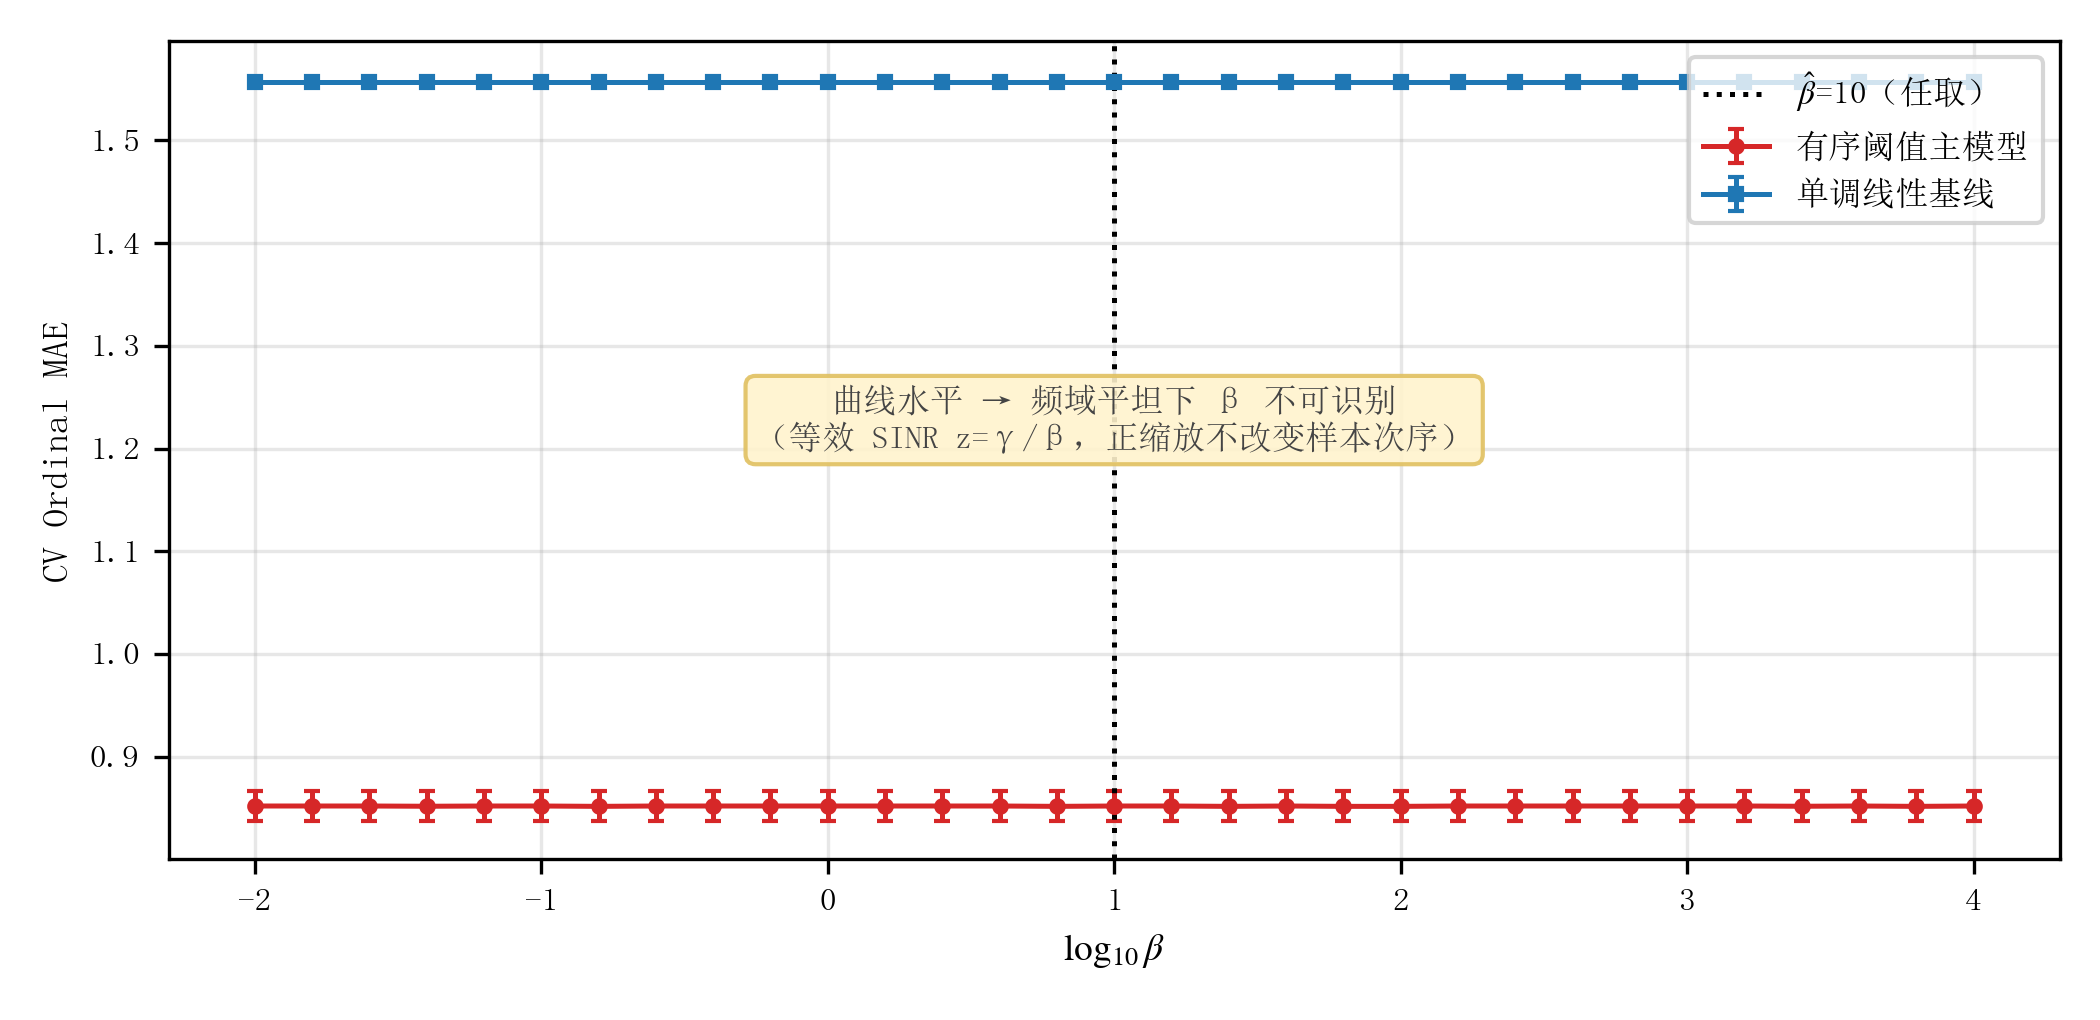
\includegraphics[width=0.72\textwidth]{problem1/output/figures/fig4_beta_cv_curve.png}
\caption{交叉验证 Ordinal MAE 随 $\log_{10}\beta$ 的变化曲线（含各折标准差）}
\label{fig:q1-beta-cv}
\end{figure}

\subsubsection{等效SINR与MCS的关系}

图~\ref{fig:q1-sinr-box} 给出了按真实 MCS 分组的等效 SINR（dB）箱线图。可以看出，各 MCS 等级的等效 SINR 中心位置整体随等级升高而右移，但相邻等级之间存在明显重叠，说明等效 SINR 对 MCS 具有显著且有序的区分能力，但并非一一对应，需要数据驱动地标定阈值。

\begin{figure}[H]
\centering
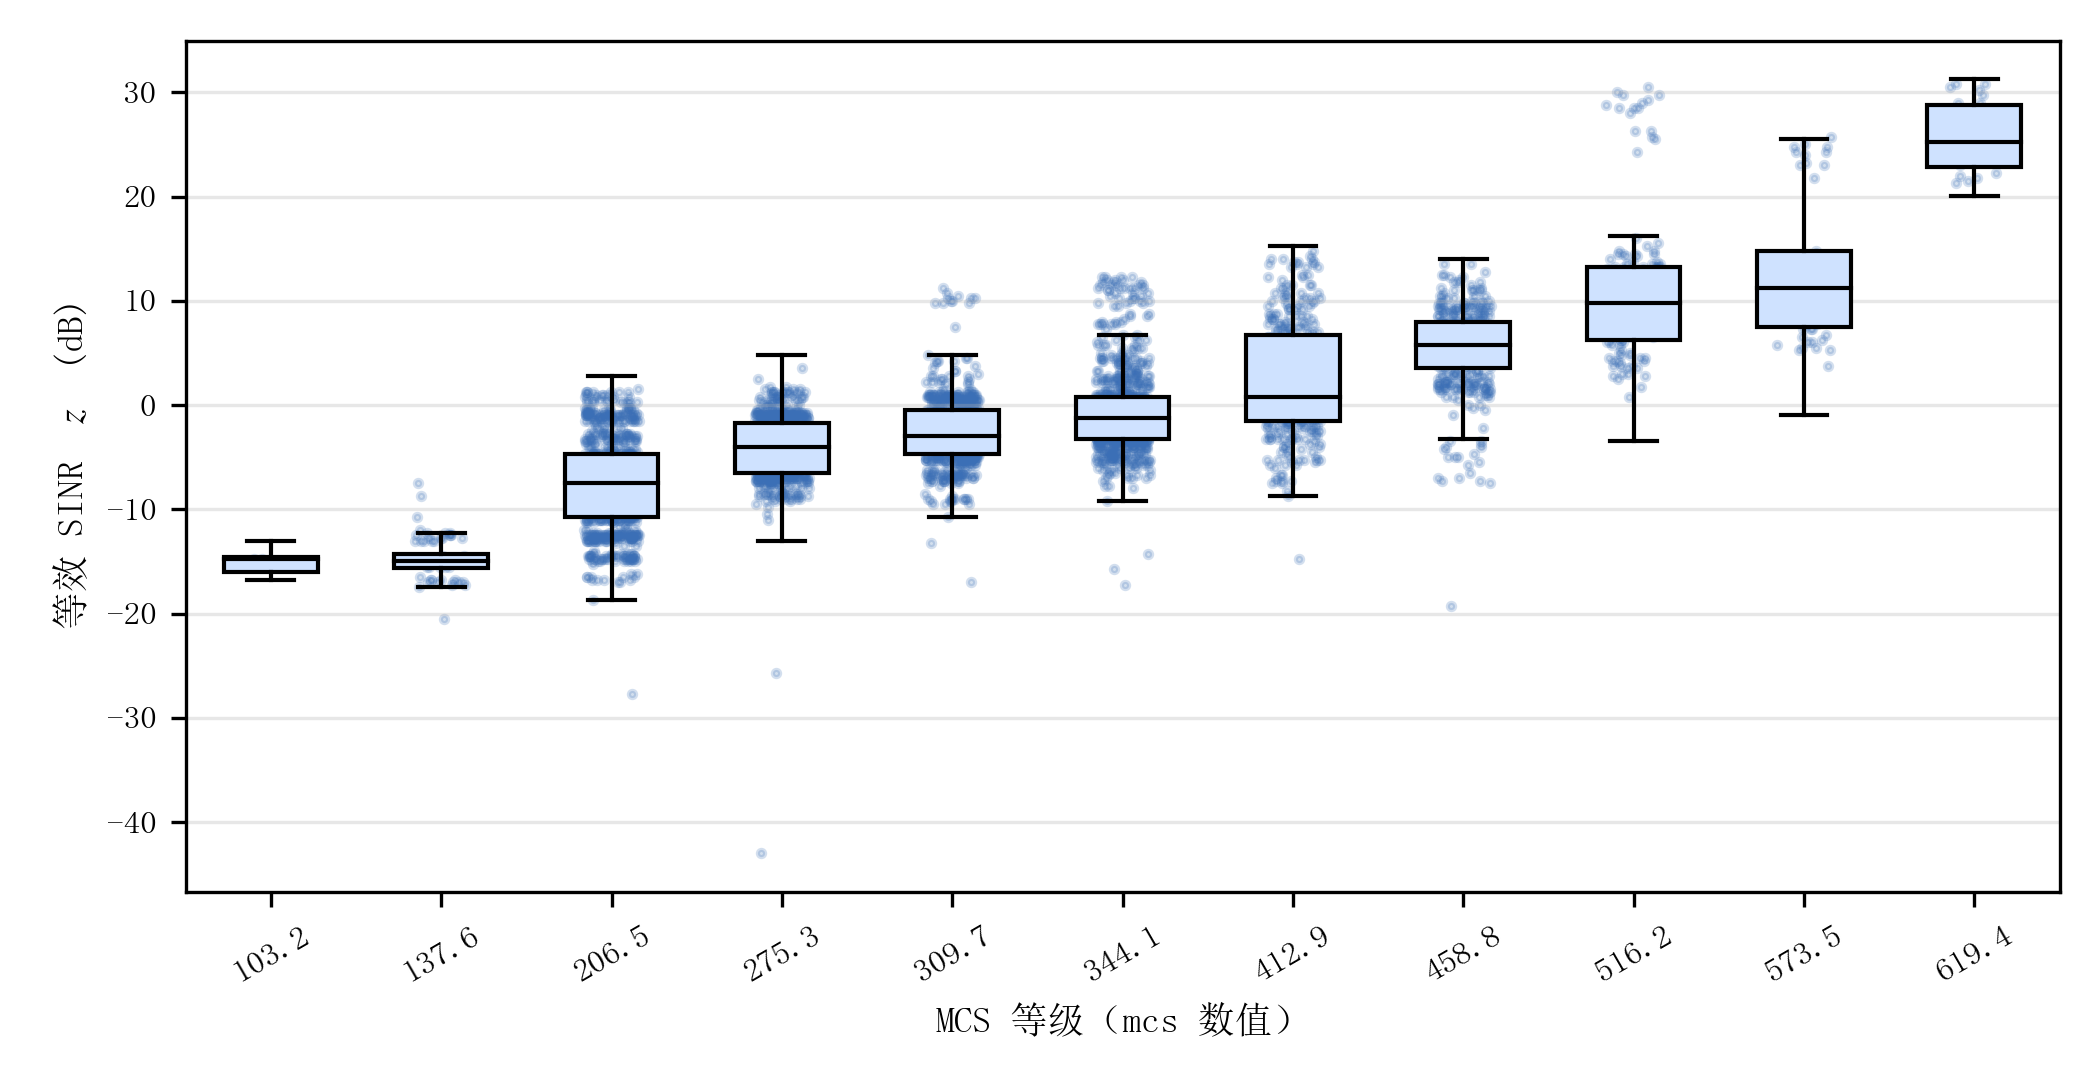
\includegraphics[width=0.75\textwidth]{problem1/output/figures/fig2_sinr_by_mcs_boxplot.png}
\caption{不同 MCS 等级的等效 SINR 分布箱线图}
\label{fig:q1-sinr-box}
\end{figure}

图~\ref{fig:q1-thresholds} 给出了训练样本的等效 SINR--MCS 散点图，并叠加了主模型的最优有序阈值（虚线）与阶梯映射函数（红色阶梯）。可见最优阈值间距明显不均：低等级区间阈值密集、高等级区间阈值稀疏，直观说明 $z\to\mathrm{MCS}$ 的映射关系并非简单等距线性，进一步印证了有序阈值结构的必要性。

\begin{figure}[H]
\centering
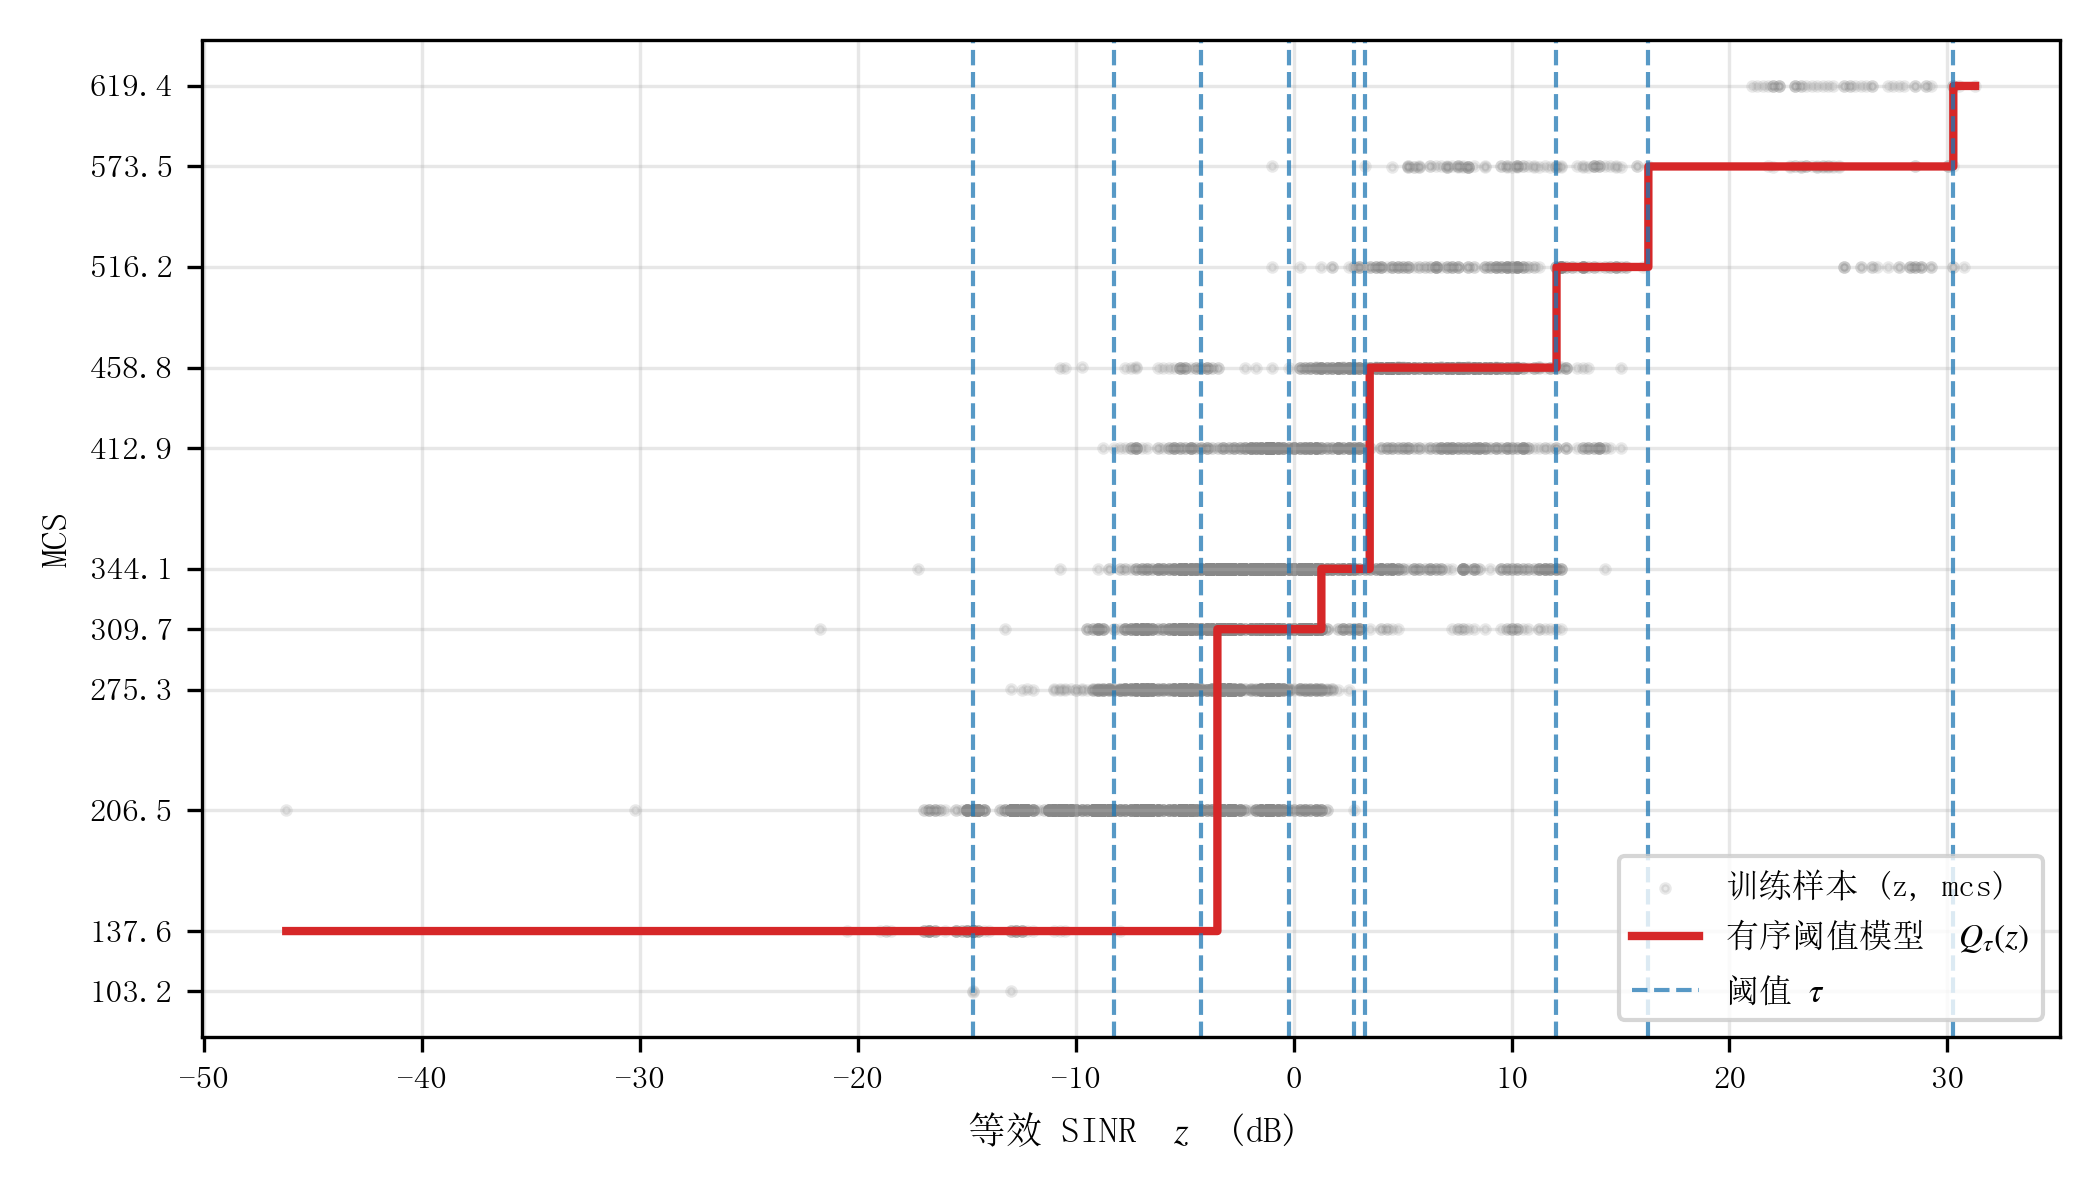
\includegraphics[width=0.75\textwidth]{problem1/output/figures/fig3_sinr_mcs_thresholds.png}
\caption{等效 SINR--MCS 散点图与最优有序阈值}
\label{fig:q1-thresholds}
\end{figure}

\subsubsection{主模型与基线对比}

两种速率映射模型在相同 5 折数据划分下的交叉验证性能如表~\ref{tab:q1-compare} 所示（mean $\pm$ std）。

\begin{table}[H]
	\centering
	\caption{两种速率映射模型的交叉验证性能}
	\label{tab:q1-compare}
	\begin{tabular}{lccc}
		\toprule
		模型 & Accuracy $\uparrow$ & Ordinal MAE $\downarrow$ & $\mathrm{Acc}_{\pm1}$ $\uparrow$ \\
		\midrule
		单调线性基线 & $0.1512\pm0.0009$ & $1.5564\pm0.0046$ & $0.5214\pm0.0007$ \\
		有序阈值主模型 & $0.3763\pm0.0083$ & $0.8520\pm0.0148$ & $0.8077\pm0.0073$ \\
		$L_2$ 等渗回归（额外对照） & $0.3636\pm0.0089$ & $0.8519\pm0.0135$ & $0.8159\pm0.0054$ \\
		\bottomrule
	\end{tabular}
\end{table}

由表~\ref{tab:q1-compare} 可见，有序阈值主模型在三项指标上全面优于单调线性基线：Accuracy 由 $0.1512$ 提升至 $0.3763$，Ordinal MAE 由 $1.5564$ 降至 $0.8520$，$\mathrm{Acc}_{\pm1}$ 由 $0.5214$ 提升至 $0.8077$。这表明不同 MCS 等级对应的等效 SINR 区间并非等距分布，采用非等距有序阈值能够更准确地刻画实际链路的阶梯式速率变化；线性模型因强制等距假设而无法适应等级间疏密不均的阈值结构。此外，$L_2$ 等渗回归作为额外对照取得了与主模型接近的性能，验证了第三层映射单调性假设的核心地位。因此，后续对验证集 B 的预测采用有序阈值主模型。

图~\ref{fig:q1-error} 给出了两种模型的等级误差 $e=c(\widehat y)-c(y)$ 分布。主模型的误差高度集中于 $e=0$ 与 $e=\pm1$，而线性基线在 $e=0$ 处比例明显更低、大误差样本更多，进一步说明主模型对 MCS 档位边界的刻画更为准确。

\begin{figure}[H]
\centering
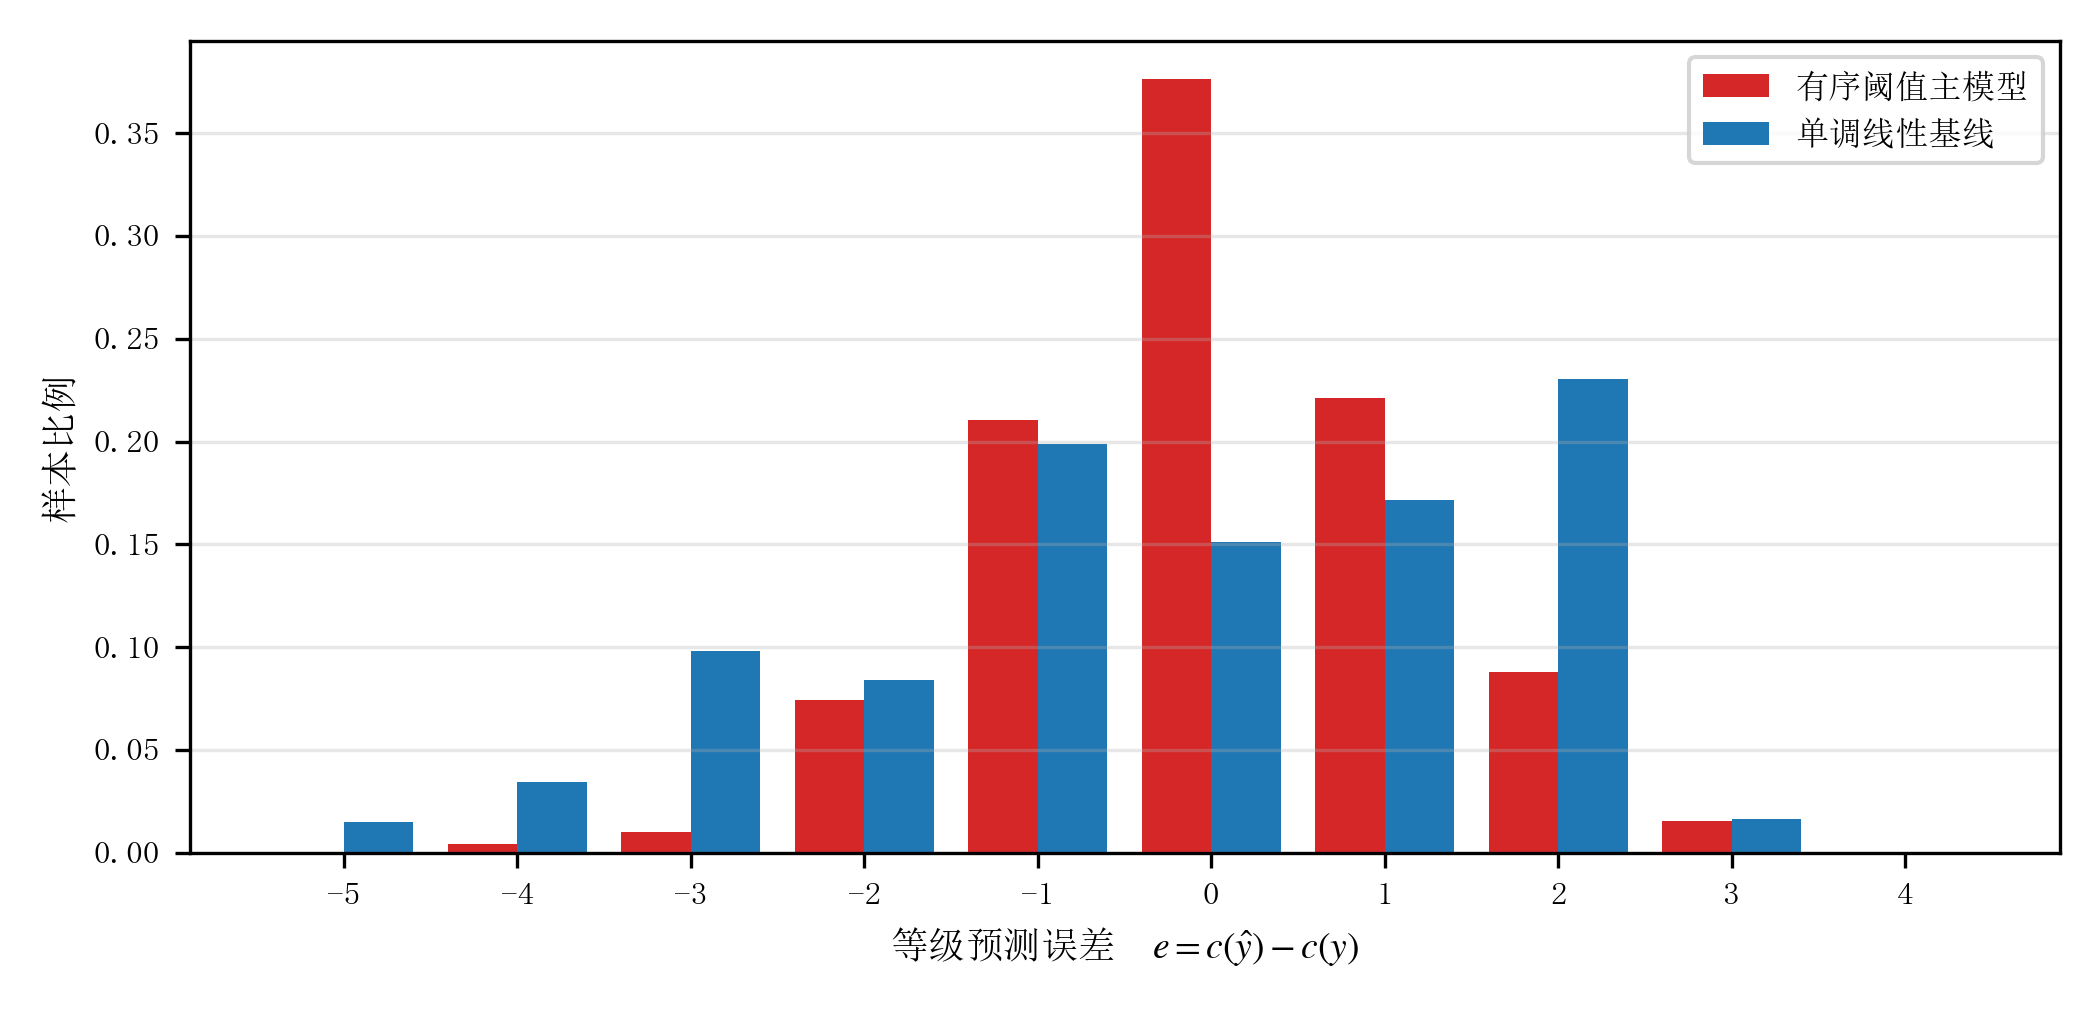
\includegraphics[width=0.75\textwidth]{problem1/output/figures/fig5_error_distribution.png}
\caption{两种模型的 MCS 等级预测误差分布（折外预测）}
\label{fig:q1-error}
\end{figure}

图~\ref{fig:q1-confusion} 给出了主模型按真实类别行归一化的混淆矩阵，其质量集中于主对角线及相邻位置，说明模型的误判几乎全部发生在相邻速率等级之间，属于等级边界处信道质量模糊造成的局部混淆，与 Ordinal MAE 和 $\mathrm{Acc}_{\pm1}$ 的评价结论一致。

\begin{figure}[H]
\centering
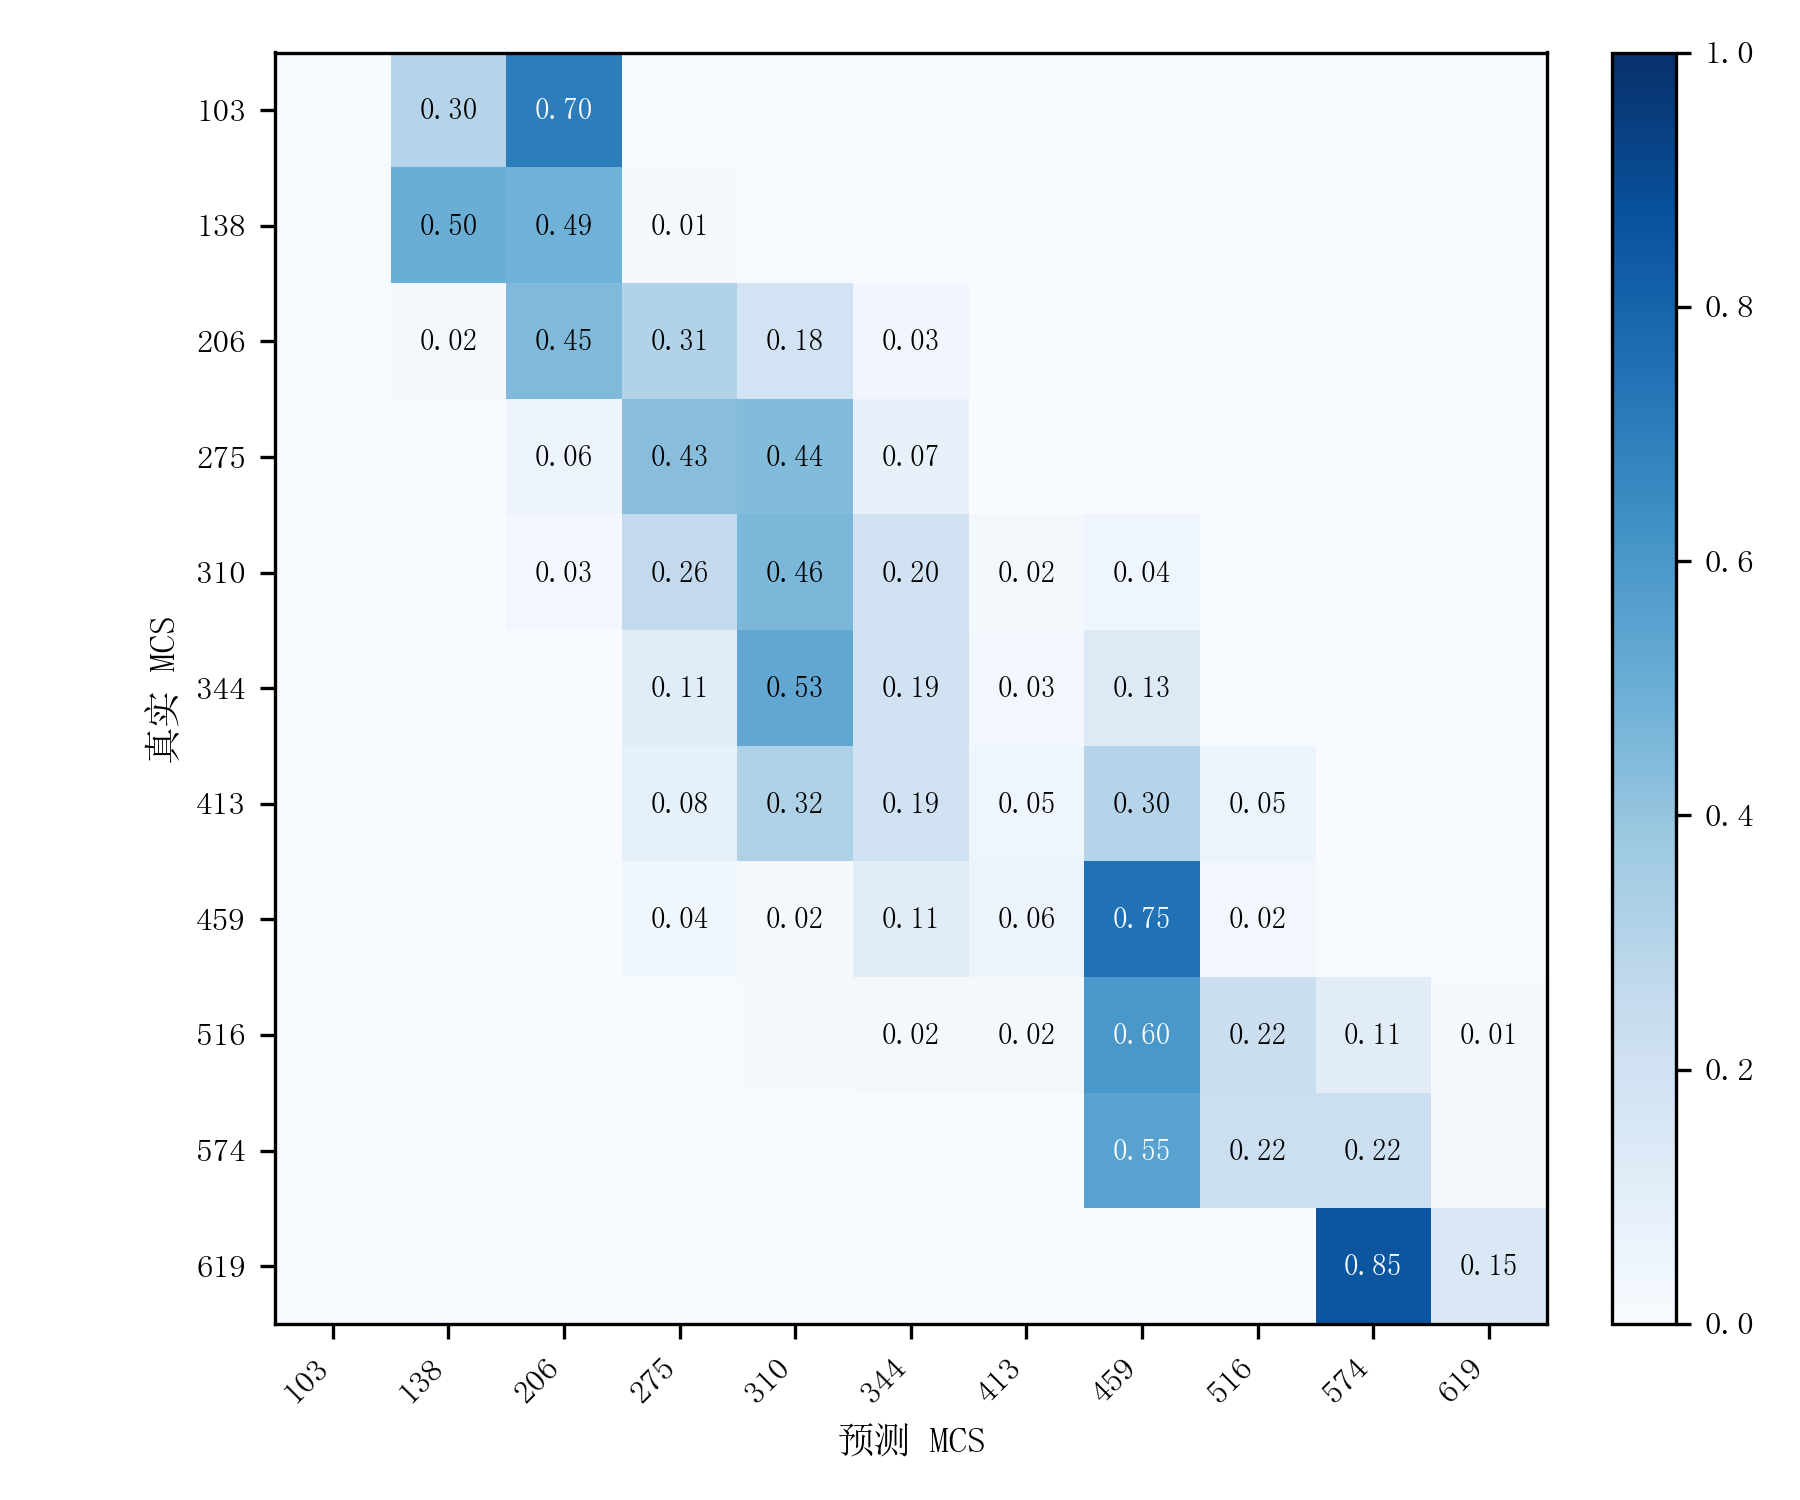
\includegraphics[width=0.75\textwidth]{problem1/output/figures/fig6_confusion_matrix.png}
\caption{有序阈值主模型的归一化混淆矩阵（折外预测）}
\label{fig:q1-confusion}
\end{figure}

\subsection{验证集B的速率预测}

利用训练集 A 的全部关闭 TxBF 样本，以交叉验证确定的 $\widehat\beta_{\mathrm{ord}}$ 重新拟合最优有序阈值 $\widehat{\boldsymbol{\tau}}$。对于验证集 B 中第 $j$ 个待预测样本，首先计算
\begin{equation}
	\gamma_{j,k}=\frac{\|H_k^{(j)}\|_F^2}{P_n^{(j)}},
	\qquad k=1,\ldots,122,
\end{equation}
再计算等效 SINR
\begin{equation}
	\boxed{
	z_j=-\ln\left[\frac{1}{122}\sum_{k=1}^{122}\exp\left(-\frac{\gamma_{j,k}}{\widehat\beta_{\mathrm{ord}}}\right)\right],
	}
	\label{eq:z-final}
\end{equation}
最终根据
\begin{equation}
	\widehat y_j=Q_{\widehat{\boldsymbol{\tau}}}(z_j)
	\label{eq:pred-final}
\end{equation}
得到预测 MCS。验证集 B 共 $20369$ 条样本，其预测结果如表~\ref{tab:q1-B} 所示（前 10 条预览，完整结果见附录）。

\begin{table}[H]
	\centering
	\caption{验证集 B 的问题一 MCS 预测结果（前 10 条预览）}
	\label{tab:q1-B}
	\begin{tabular}{clcc}
		\toprule
		样本编号 & 终端标识 & 等效 SINR（dB） & 预测 MCS \\
		\midrule
		$0$ & 341c-f0d4-70be & $-0.979$ & $309.7$ \\
		$1$ & 341c-f0d4-70be & $-8.979$ & $206.5$ \\
		$2$ & 341c-f0d4-70be & $-7.229$ & $275.3$ \\
		$3$ & 341c-f0d4-70be & $-6.729$ & $275.3$ \\
		$4$ & 341c-f0d4-70be & $-4.479$ & $275.3$ \\
		$5$ & 341c-f0d4-70be & $-4.979$ & $275.3$ \\
		$6$ & 341c-f0d4-70be & $-8.729$ & $206.5$ \\
		$7$ & 341c-f0d4-70be & $-4.979$ & $275.3$ \\
		$8$ & 341c-f0d4-70be & $-6.479$ & $275.3$ \\
		$9$ & 341c-f0d4-70be & $-7.229$ & $275.3$ \\
		$\vdots$ & $\vdots$ & $\vdots$ & $\vdots$ \\
		\bottomrule
	\end{tabular}
\end{table}

\subsection{本问小结}

针对关闭 TxBF 的 MIMO-OFDM 链路，本文首先依据 CSI 和底噪信息计算 122 个载波单元的 SINR，再利用 EESM 将高维载波状态压缩为单一等效 SINR。由于数据中缺少真实等效 SINR 标签，本文没有采用相互独立的两阶段参数拟合，而是直接以最终 MCS 预测误差为目标，对 EESM 参数和速率映射参数进行联合标定。

在速率映射层，本文根据 MCS 的有序离散特征建立非等距有序阈值模型，并设置单调线性模型作为基线。求解时，将原联合优化分解为一维 EESM 参数搜索和内层参数求解：主模型使用动态规划获得固定 $\beta$ 下的最优阈值，线性基线使用加权最小二乘解析求解。

实验结果表明：实测信道频域平坦，EESM 参数 $\beta$ 在数据上不可识别，等效 SINR 退化为载波级 SINR 的比例缩放；有序阈值主模型在 5 折交叉验证中取得 Accuracy $=0.3763$、Ordinal MAE $=0.8520$、$\mathrm{Acc}_{\pm1}=0.8077$，全面优于单调线性基线（$0.1512$/$1.5564$/$0.5214$），验证了非等距有序阈值结构对刻画阶梯式速率映射的必要性。最终利用主模型完成了验证集 B 共 $20369$ 条链路的 MCS 索引预测。

\section{问题二 xxx}
\subsection{问题描述和分析}
问题的分析问题的分析问题的分析问题的分析问题的分析问题的分析问题的分析问题的分析问题的分析问题的分析问题的分析问题的分析问题的分析问题的分析。
\subsection{模型建立与求解}
模型建立与求解模型建立与求解模型建立与求解模型建立与求解模型建立与求解模型建立与求解模型建立与求解模型建立与求解模型建立与求解模型建立与求解模型建立与求解。

\section{问题三 xxx}
\subsection{问题描述和分析}
问题的分析问题的分析问题的分析问题的分析问题的分析问题的分析问题的分析问题的分析问题的分析问题的分析问题的分析问题的分析问题的分析问题的分析。
\subsection{模型建立与求解}
模型建立与求解模型建立与求解模型建立与求解模型建立与求解模型建立与求解模型建立与求解模型建立与求解模型建立与求解模型建立与求解模型建立与求解模型建立与求解。

\section{问题四 xxx}
\subsection{问题描述和分析}
问题的分析问题的分析问题的分析问题的分析问题的分析问题的分析问题的分析问题的分析问题的分析问题的分析问题的分析问题的分析问题的分析问题的分析。
\subsection{模型建立与求解}
模型建立与求解模型建立与求解模型建立与求解模型建立与求解模型建立与求解模型建立与求解模型建立与求解模型建立与求解模型建立与求解模型建立与求解模型建立与求解。

\section{模型的评价}
\subsection{模型的优点}
模型的优点模型的优点模型的优点模型的优点模型的优点模型的优点模型的优点模型的优点模型的优点模型的优点模型的优点模型的优点模型的优点模型的优点。
\subsection{模型的缺点}
模型的缺点模型的缺点模型的缺点模型的缺点模型的缺点模型的缺点模型的缺点模型的缺点模型的缺点模型的缺点模型的缺点模型的缺点模型的缺点模型的缺点。



\section{写作参考格式}
写作过程中可能要用到一些格式参考，正式写作的时候，可以直接将这一章删掉即可。

\textbf{无序列表格式}
\begin{itemize}
\item 无序列表1
\item 无序列表2
\item 无序列表3
\item 无序列表4
\end{itemize}


\textbf{表格格式}

\begin{tabular}{cc}
 \hline
 \makebox[0.4\textwidth][c]{符号}	&  \makebox[0.5\textwidth][c]{意义} \\ \hline
 D	    & 宽度（cm） \\ \hline
 L	    & 长度（cm）  \\ \hline
\end{tabular}

%三线表

\begin{table}[!htp]
	\newcolumntype{L}{X}
	\newcolumntype{C}{>{\centering \arraybackslash}X}
	\newcolumntype{R}{>{\raggedright \arraybackslash}X}
	\centering
	\caption{某校学生升高体重样本}
	\label{tab2:heightweight}
	\begin{tabularx}{0.9\textwidth}{CCCC}  %c的数量表示列数
		\toprule
		序号&年龄&身高&体重\\
		\midrule  %添加中间的线，其余同理
		1&14&156&42\\
		2&16&158&45\\
		3&14&162&48\\
		4&15&163&50\\
		%\cmidrule{2-4}
		平均&15&159.75&46.25\\
		\bottomrule
	\end{tabularx}
\end{table}

%多图并排（模板示例，图片文件不存在，已注释）
%\begin{figure}[!htp]
%	\centering
%	\subfloat[Arabic numerals]{\includegraphics[width=0.4\textwidth]{image1}}\qquad
%	\subfloat[Arabic numerals]{\includegraphics[width=0.4\textwidth]{image2}} \\
%	\subfloat[Arabic numerals]{\includegraphics[width=0.4\textwidth]{image3}}\qquad
%	\subfloat[Arabic numerals]{\includegraphics[width=0.4\textwidth]{image4}}
%	\caption{多图示例}
%\end{figure}
%
%\textbf{图片格式}
%\begin{figure}[h]
%\centering
%\includegraphics[width=5cm]{xxx.jpg}
%\caption{图片标题}
%\end{figure}
\newpage
\section{参考文献}
%参考文献
\begin{thebibliography}{1.2}%宽度9
\setlength{\itemsep}{-2mm}
 \bibitem{bib:one} 
 韩中庚. 数学建模方法及其应用[M]. 高等教育出版社, 2005.
 \bibitem{bib:two}
 韩中庚. 数学建模方法及其应用[M]. 高等教育出版社, 2005.
  \bibitem{bib:two}
 韩中庚. 数学建模方法及其应用[M]. 高等教育出版社, 2005.
\end{thebibliography}

\newpage
%附录
\appendix
\section{程序代码}
%设置不同语言即可。
\begin{lstlisting}[language=Matlab] 
kk=2;[mdd,ndd]=size(dd);
while ~isempty(V)
[tmpd,j]=min(W(i,V));tmpj=V(j);
for k=2:ndd
[tmp1,jj]=min(dd(1,k)+W(dd(2,k),V));
tmp2=V(jj);tt(k-1,:)=[tmp1,tmp2,jj];
end
tmp=[tmpd,tmpj,j;tt];[tmp3,tmp4]=min(tmp(:,1));
if tmp3==tmpd, ss(1:2,kk)=[i;tmp(tmp4,2)];
else,tmp5=find(ss(:,tmp4)~=0);tmp6=length(tmp5);
if dd(2,tmp4)==ss(tmp6,tmp4)
ss(1:tmp6+1,kk)=[ss(tmp5,tmp4);tmp(tmp4,2)];
else, ss(1:3,kk)=[i;dd(2,tmp4);tmp(tmp4,2)];
end;end
dd=[dd,[tmp3;tmp(tmp4,2)]];V(tmp(tmp4,3))=[];
[mdd,ndd]=size(dd);kk=kk+1;
end; S=ss; D=dd(1,:);
 \end{lstlisting}


\end{document} 
